\documentclass[sigconf,screen]{acmart}

\settopmatter{printacmref=false}
\renewcommand\footnotetextcopyrightpermission[1]{}
\pagestyle{plain}
\setcopyright{none}
\acmConference[SIGGRAPH Posters]{ACM SIGGRAPH 2027 Posters}{2027}{}
\acmISBN{}
\acmDOI{}
\acmPrice{}

\usepackage{amsmath}
\usepackage{booktabs}
\usepackage{graphicx}

\begin{document}

\title{Exact Deployment Range and Certified Design for Kirigami on Arbitrary Planar Graphs}

\author{Emre Dayanga\c{c}}
\affiliation{%
  \institution{Affiliation placeholder}
  \country{}
}

\begin{abstract}
We extend the uniformly deployable kirigami framework of Segall, Ren and
Sorkine-Hornung with an exact kinematic layer and a point-selection rule inside
their linear shape space $X=X_0+\Phi t$. We prove: (i) along the uniform branch
every vertex follows $Y(\theta)=\cos(\theta/2)\,C(X)+\sin(\theta/2)\,S(X)$ with
$C,S$ linear in $X$, and the branch never locks; (ii) every contact predicate is
a first harmonic $p+q\cos\theta+r\sin\theta$ with coefficients quadratic in $X$,
so the collision-free range $\Theta_{\max}$ is a minimum over closed-form
admissible roots, where grazes shift the naive minimum by up to $1.047$\,rad;
(iii) the certificate $\textsc{pos}\wedge\textsc{nooverlap}(\varepsilon/2)\wedge
\textsc{noroot}(\varepsilon)$ implies $\Theta_{\max}\ge\varepsilon$, is exact
below the first graze and is not complete. On 3{,}113 designs the exact
$\Theta_{\max}$ agrees with a bisection referee at $10^{-5}$ on all 3{,}113
(worst gap $3.8\times10^{-9}$); the certificate holds on 2{,}150 with 0
violations. On 400 random Voronoi, Delaunay and quad designs (median $|F|=332$)
the default Eq.~(6) projection gives $\Theta_{\max}=0$ on all 400; we trace this
to reflex corners the projection introduces (1{,}966 of 1{,}968 jammed balanced
vertices) and certify by Farkas duality that no first-order flex avoids the
$0^{+}$ contacts on 96 of 100. Replacing the proximity objective by a two-stage
margin-then-range maximisation under convexity and split-outward barriers, in the
same shape space, gives $\Theta_{\max}>0$ on 307 of the 400 (306 certified, 185 of
200 graphs, up to $\pi$). For periodic patterns we prove
$J(\theta)=\cos(\theta/2)I+\sin(\theta/2)K$ with $K$ affine in $t$, so
first-order conformality holds for every $\theta$.
\end{abstract}

\keywords{kirigami, auxetic metamaterials, computational fabrication, rigidity}

\begin{teaserfigure}
  \centering
  \begin{minipage}[t]{0.32\linewidth}
    \centering
    \includegraphics[height=0.68in]{figs/teaser_closed.png}\\[2pt]
    {\footnotesize $\theta = 0$}
  \end{minipage}\hfill
  \begin{minipage}[t]{0.32\linewidth}
    \centering
    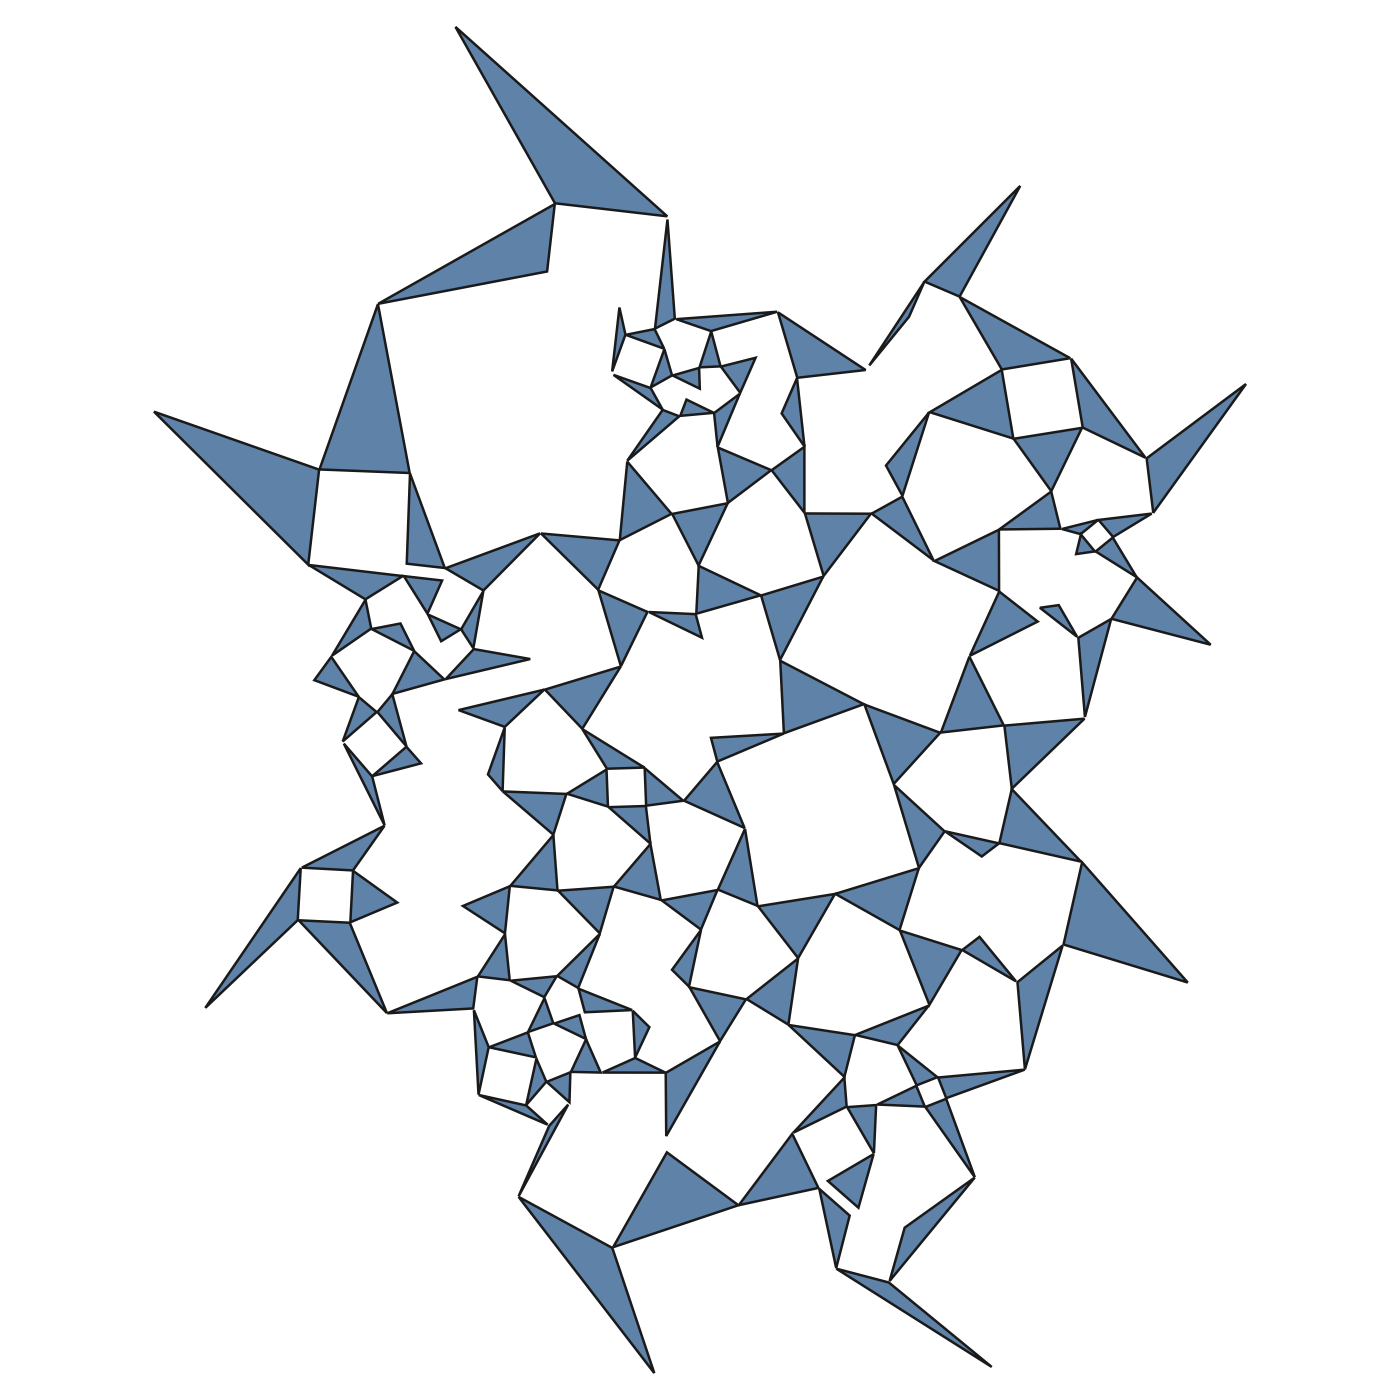
\includegraphics[height=0.68in]{figs/teaser_half.png}\\[2pt]
    {\footnotesize $\theta = \Theta_{\max}/2$}
  \end{minipage}\hfill
  \begin{minipage}[t]{0.32\linewidth}
    \centering
    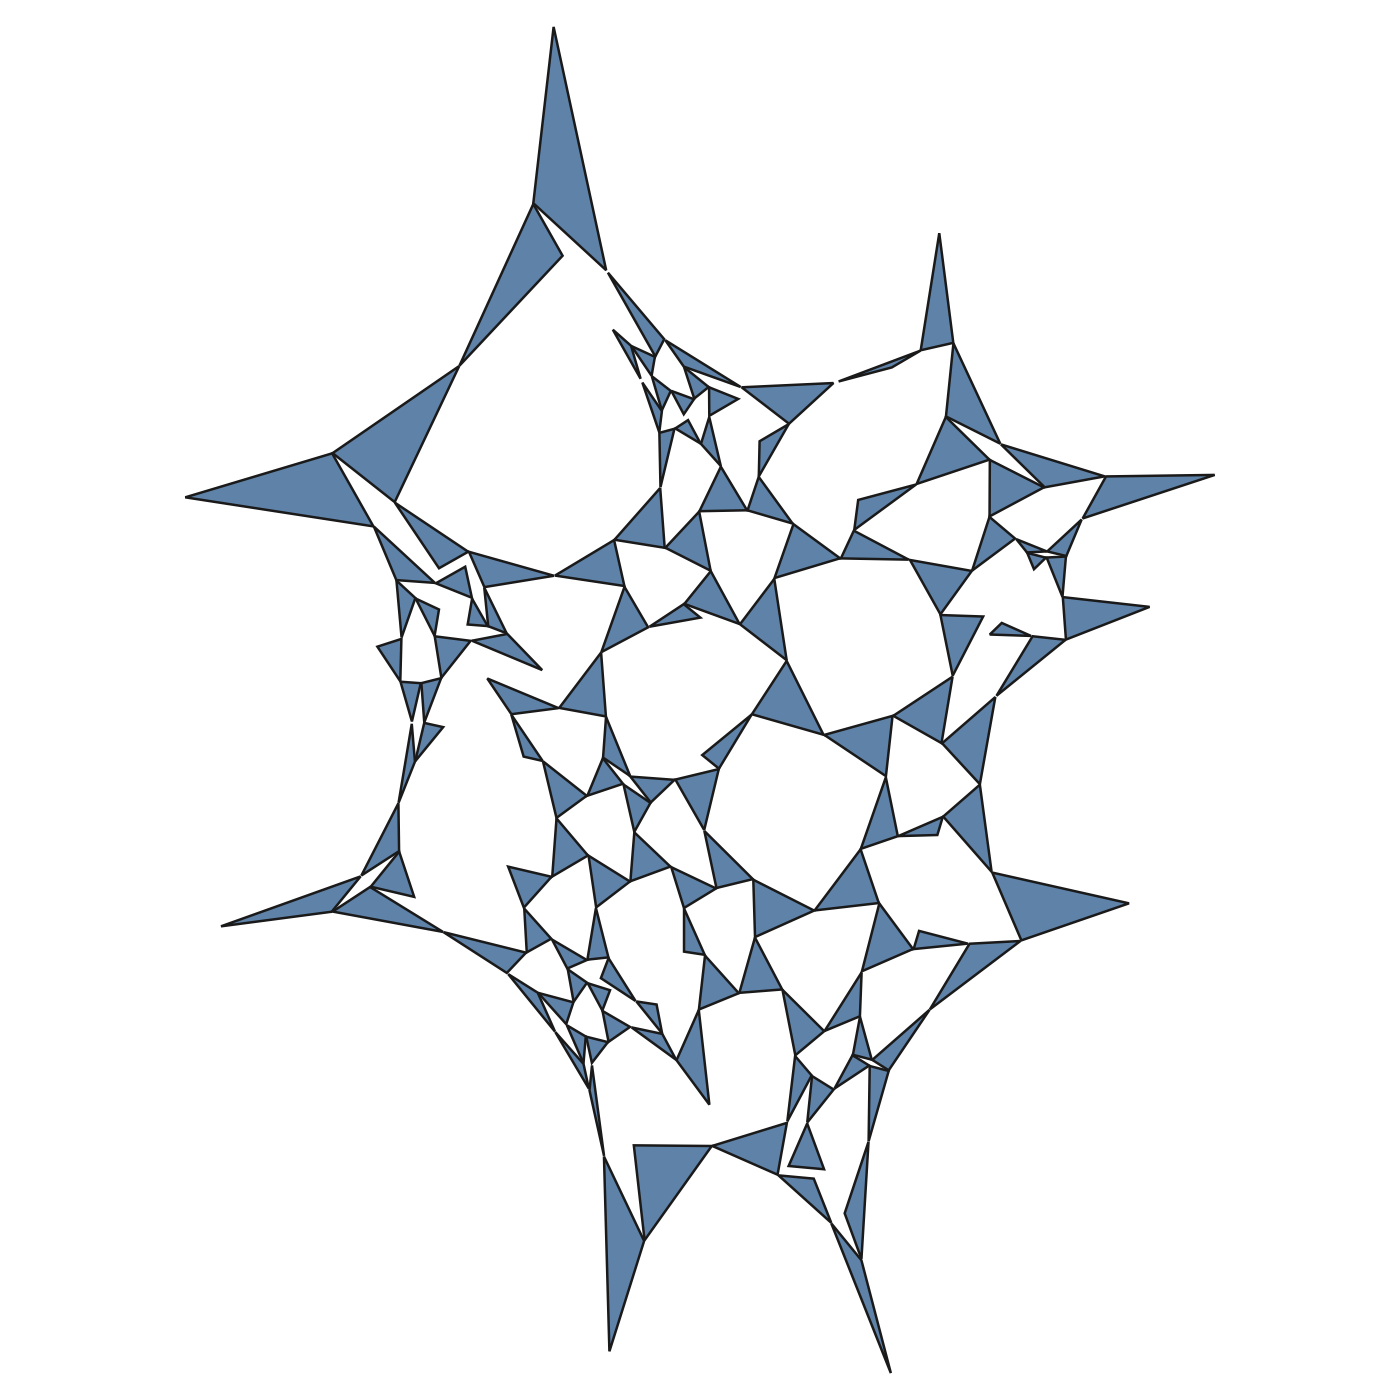
\includegraphics[height=0.68in]{figs/teaser_open90.png}\\[2pt]
    {\footnotesize $\theta = 0.9\,\Theta_{\max}$}
  \end{minipage}
  \caption{A certified design from our range-maximising constrained embedding, on a
  random Delaunay graph ($|F|=130$ faces, $|V|=71$ vertices, 18 split cut edges),
  at $\theta=0$, $\Theta_{\max}/2$ and $0.9\,\Theta_{\max}$. Here
  $\Theta_{\max}=\pi$: it opens fully, certified collision-free, no inverted faces.
  The default Eq.~(6) projection gives $\Theta_{\max}=0$ here.}
  \label{fig:teaser}
\end{teaserfigure}

\maketitle

\section{Introduction}

Segall, Ren and Sorkine-Hornung~\cite{Segall2026} give a linear shape space
$\mathcal{X}$ of \emph{uniformly deployable} kirigami on arbitrary planar graphs:
a corner-hinged rigid tiling of a 3-connected planar graph whose faces all rotate
by the same angle, generalising their tessellation-based
predecessor~\cite{Segall2025}. Their Limitation~1 names the gap: ``uniform
deployability does not guarantee a large collision-free deployment range;
self-intersections may occur at small opening angles \dots\ Developing geometric
characteristics for favorable deployment behavior directly from the embedding
remains an open problem.''

We take that up inside their framework. Everything below lives in their shape
space $\mathcal{X}$ and cut/hole formalism; we add an exact kinematic layer and a
point-selection rule. The range is closed-form and certifiable, turning the open
problem into a predicate; optimising it yields embeddings that deploy.

\section{Exact kinematics and a sound certificate}

\paragraph{Deployment path (Lemma).} With $\theta$ the opening angle, every vertex
of the cut mesh moves along
\begin{equation}
  Y(\theta) \;=\; \cos(\theta/2)\,C(X) \;+\; \sin(\theta/2)\,S(X),
  \label{eq:path}
\end{equation}
with $C$ and $S$ \emph{linear} in the flat design coordinates $X$: the
Tay--Whiteley body-and-hinge motion assignment~\cite{Katoh2009} made trig-linear
and specialised to corner-hinged tilings, with the half-angle magnitude
anticipated, under two extra hypotheses, by Acu\~na et al.~\cite{Acuna2022}. It is
a lemma.

\paragraph{Exact first contact.} Substituting~\eqref{eq:path} into any
signed-area, vertex-edge or edge-edge predicate gives a single first harmonic
$p+q\cos\theta+r\sin\theta$ with coefficients \emph{quadratic in $X$}, so the
collision-free range is a minimum over closed-form roots. The subtlety is
degeneracy: a vertex-vertex touch can be a \emph{graze} rather than an
overlap, and the candidate list must separate the two. On the hexagon
of~\cite{Segall2026} the first contact angle is $\theta_1=\pi/3$ while
$\Theta_{\max}=2\pi/3$, refining the implicit reading
$\Theta_{\max}=\min_e\beta_e$ of their per-hinge bound. We prove one
direction, $\Theta_{\max}\le\min(\min_e\beta_e,\pi)$; the reverse is measured on 8
patterns, not proved. Dropping the graze clause errs by up to $1.047$~rad on 5
of 187 designs; Grima et al.~\cite{Grima2012} treat only the hinge-adjacent case.

\paragraph{Certificate.} Let $\textsc{pos}$ assert positive signed areas at
$\theta=0$, $\textsc{nooverlap}(\varepsilon/2)$ no face-face overlap at the
midpoint, and $\textsc{noroot}(\varepsilon)$ no admissible contact root in
$(0,\varepsilon)$; their conjunction implies $\Theta_{\max}\ge\varepsilon$. Scope
matters: it is \emph{exact} for $\varepsilon$ below the first graze, a strict
inner approximation above it, and \emph{incomplete} --- the hexagon at
$\varepsilon=\pi/2$ has range and fails it.

\paragraph{Validation (E1).} $N=3{,}113$ designs (1{,}660 authored, 1{,}322
jittered, 131 random; 13 families, both orientation rules): exact
$\Theta_{\max}$ vs.\ a tolerance-independent bisection referee agrees
$3{,}113/3{,}113$ at $10^{-5}$; at $\varepsilon=0.006$ the certificate holds on
2{,}150 designs, 0 violations, and exactly those 2{,}150 have
$\Theta_{\max}\ge\varepsilon$.

\section{Characterising the design space at scale}

$\mathcal{X}$ is rich, but on 200 random Voronoi, Delaunay and quad graphs
($|F|\in[101,793]$, median $332.5$), under both orientation rules, no variant of
the default Eq.~(6) projection we tried lands on a deployable point
(Table~\ref{tab:baseline}).

\begin{table}[t]
  \caption{Certified deployable designs, random graphs.}
  \label{tab:baseline}
  \footnotesize
  \begin{tabular}{lr}
    \toprule
    strategy & certified deployable \\
    \midrule
    default Eq.~(6) projection, sampled and projected & 0 / 400 \\
    four $0^{+}$-repair strategies & 0 / 400 \\
    boundary rows dropped & 1 / 400 (refereed) \\
    non-uniform expansive-cone LP & 0 / 100 \\
    authors' native pipeline (partial) & 0 / 172 completed \\
    \midrule
    \textbf{ours (range-maximising embedding)} & \textbf{306 / 400} \\
    \bottomrule
  \end{tabular}
\end{table}

\paragraph{The mechanism is the selected point, not the graph.} The input embeddings
have \emph{zero} non-convex face corners; the projected embeddings have 22{,}103
of 156{,}220, and of 1{,}968 balanced pure vertices with a non-positive $0^{+}$
margin, 1{,}966 sit at a reflex corner. At a convex corner the separation margin
is a disjunction $\max(-g_1,-g_2)$ over the two incident half-edges; at a reflex
corner it becomes a conjunction $\min(-g_1,-g_2)$, which is what fails. We found
no counterpart to this mechanism in the literature.

\paragraph{Emptiness beyond uniform flexes.} Asking for \emph{any} first-order
flex in the kernel avoiding the $0^{+}$ contacts is a linear program, in the
spirit of the expansion cone of Rote, Santos and Streinu~\cite{Rote2003} but
indexed by the cuts. It is infeasible: after an independent re-verification of
the dual, 96 of 100 designs at the initial embedding and 99 of
100 at the projected one carry sound Farkas certificates with residual below
$10^{-6}$. \textbf{Caveat:} these cover 4 visited branch charts of $2^{2338}$,
not all.

\paragraph{Scope of the comparison.} The reference implementation, run on 193 of
the 200 graphs (573 of 600 runs; 362 timeouts, 39 crashes), opens 0 of its 172
completed outputs by our exact scan; its own collision test reports 5, whose
contacts our scan finds it misses.

\section{Range-maximising constrained embedding}

We keep their shape space, $X(t)=X_0+\Phi t$, and their linear system, and change
only the objective. Two stages run inside that null space under convexity and
split-outward barriers. \textbf{Stage~A} maximises the $0^{+}$ deployment margin
$m(X)=\min(\min_e q_e,\min_j \mu_j)/\mathrm{med}^2$ via a log-sum-exp softmin
proved to lower-bound $m$ for every $t$; the reported $m$ is the exact minimum.
\textbf{Stage~B} maximises the exact $\Theta_{\max}$ in a shrinking trust region
with exact rejection.

On the identical 400 designs: 307 deployable (76.8\%), all 307 refereed, 306
certified, 207 with $\varepsilon_{\max}\ge0.1$~rad, median $\varepsilon_{\max}$
$0.254$~rad, maximum $\pi$. Taking the better orientation rule per graph, 185 of
the 200 graphs deploy. Two proximity-objective arms on the same population give
36/400 and 27/400: the jump comes from the objective, not the population. Yield is not scale-free (Figure~\ref{fig:yield}). The
convexity primitive is not new --- Choi, Dudte and Mahadevan~\cite{Choi2019} use
the same corner inequality --- but applying it inside a linear null space, paired
with a split-inward condition on duplicated vertices, has no counterpart we found.

\begin{figure}[t]
  \centering
  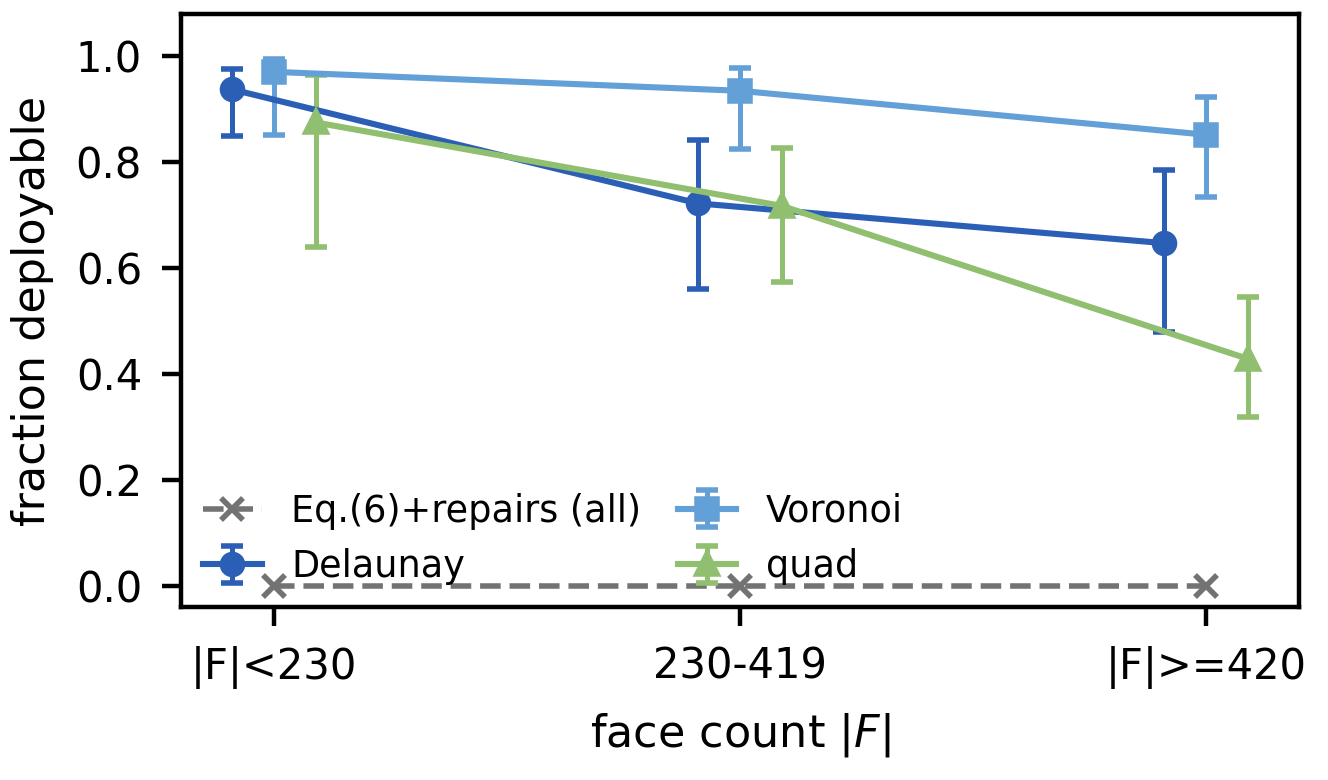
\includegraphics[width=0.56\columnwidth]{figs/fig_yield_poster.png}
  \caption{Yield versus face count, $N=400$ designs (200 graphs $\times$ 2
  orientation rules, pooled per family), Wilson 95\% intervals. The default
  projection plus our four repairs is identically zero in every bin and family,
  so it contributes no deployed design to plot.}
  \label{fig:yield}
\end{figure}

\section{Periodic patterns}

For a periodic pattern the deployment Jacobian is
$J(\theta)=\cos(\theta/2)I+\sin(\theta/2)K$ with $K$ affine in the shape
coordinate, so first-order conformality at $\theta=0$ propagates to \emph{every}
$\theta$: residual $\le10^{-16}$ over 200 angles, 25 of 25 designable patterns.
This proves as an identity the behaviour~\cite{Segall2026} reports empirically.

\section{Limitations}

Our constructive results hold under an \emph{added} convexity and split-inward
constrained embedding, not the default Eq.~(6) pipeline, on one 200-graph
population, with median certified opening $0.254$~rad, from a non-convex heuristic
with no completeness guarantee. Slivers remain a caveat: Figure~\ref{fig:teaser} has a minimum face-corner angle of $5.07^\circ$
and 3 sliver corners of 390 --- the short edges and sharp angles Limitation~1 also
names. The certificate is an inner approximation above
the first graze; completeness is false. Our population has median $|F|=332$ while
every reference case in~\cite{Segall2026} has $|F|\le97$, and that paper claims
combinatorial generality, not a success rate, so our measurement concerns a
scale it never tests. The concurrent preprint~\cite{Jiang2026} has no collision content.

{\footnotesize\setlength{\bibsep}{0pt}\bibliographystyle{ACM-Reference-Format}
\bibliography{refs}}

\end{document}
